%Correctness
\section{Correctness}
\subsection{The Graph Structure}
\begin{figure}[htb]
    \centering
    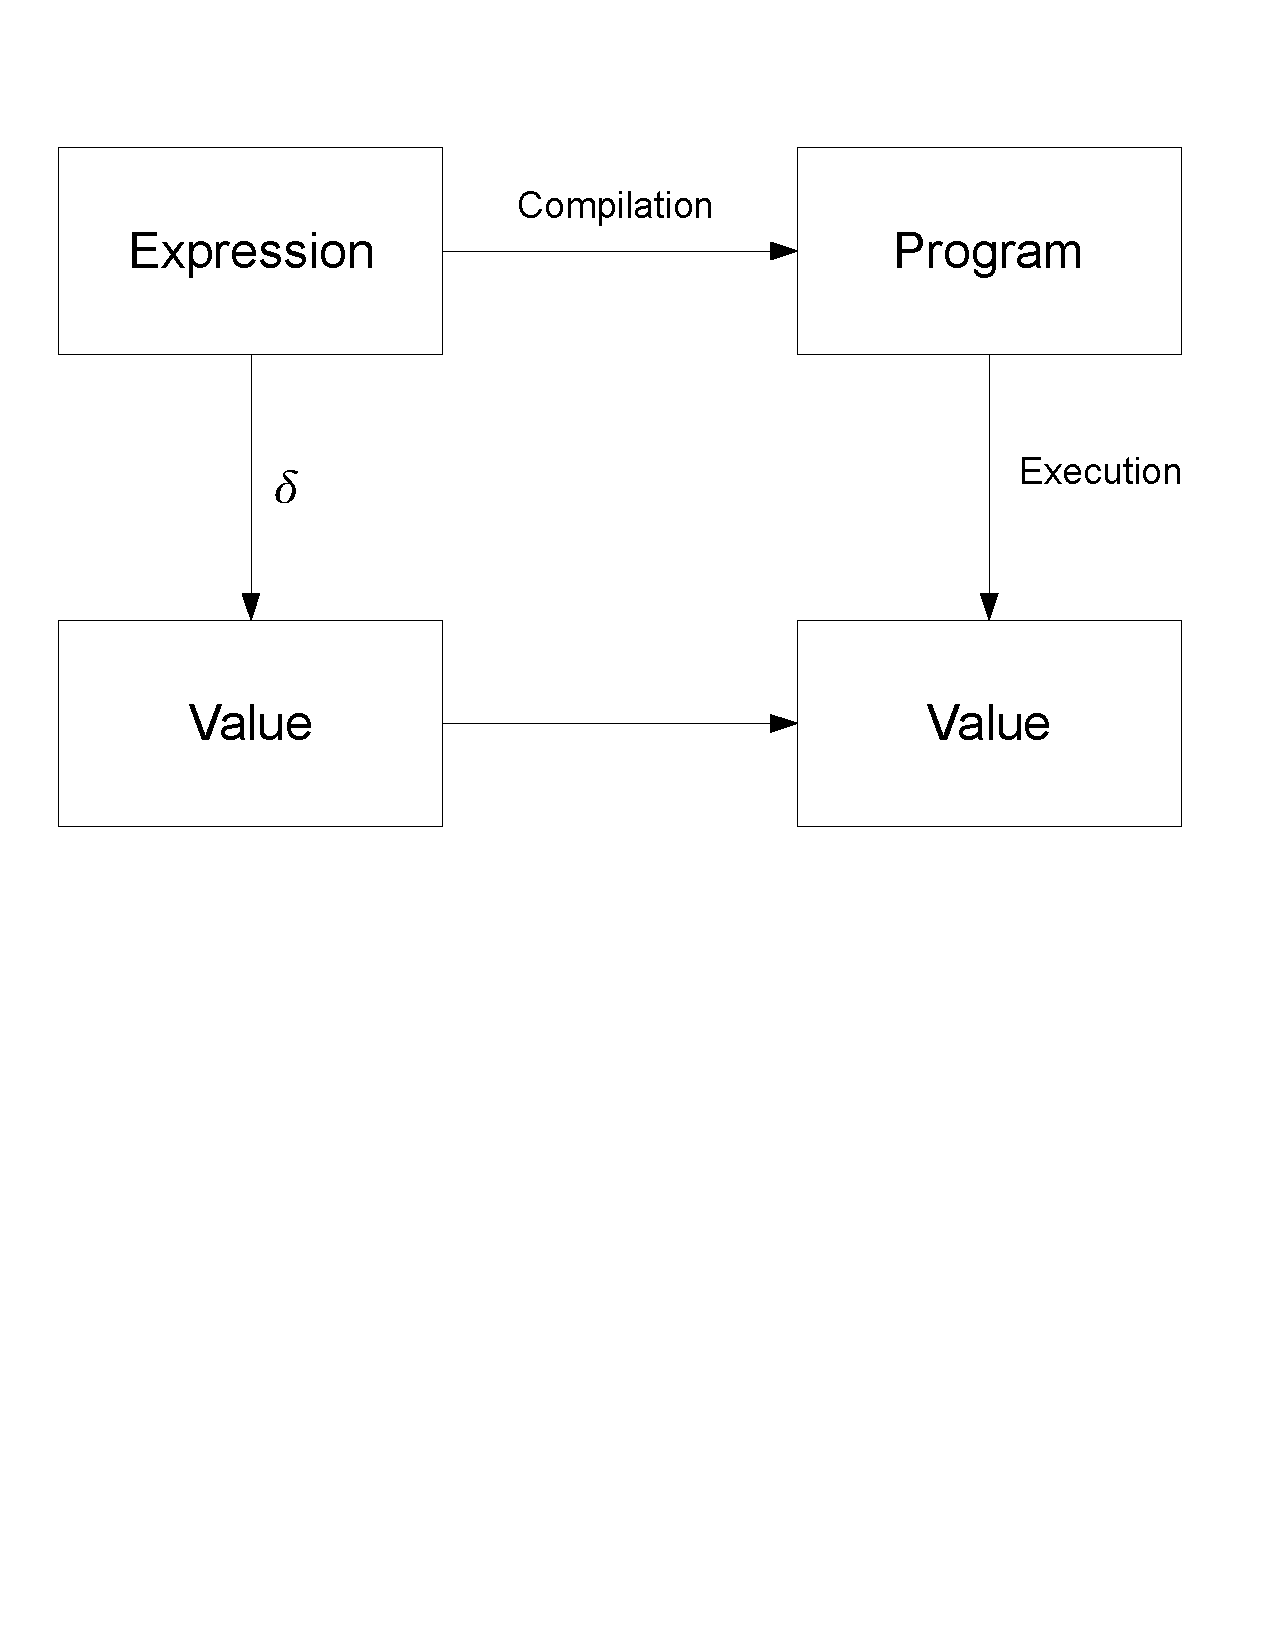
\includegraphics[trim= 10mm 120mm 10mm 10mm, clip, width=250px]{./images/correctness_graph1.pdf}
    \caption{Code Transformations}
    \label{fig:correctness_graph1}
\end{figure}
The graph structure chosen is simple directed graph in which the syntax and semantics are discussed in detail in sections \ref{sec:statechartsyn}, \ref{sec:statechartsem} respectively. Our program preforms transformations on the diagram to form code constructs. In order to show correctness we will demonstrate that our transformations follow figure \ref{fig:correctness_graph1}. Figure \ref{fig:correctness_graph1} essentially says that a simulated evaluation of each expression ($\delta$) to a value will be equivalent to the actual executed program of the same value. In addition we also need to justify the program structure

\begin{figure}[htb]
    \centering
    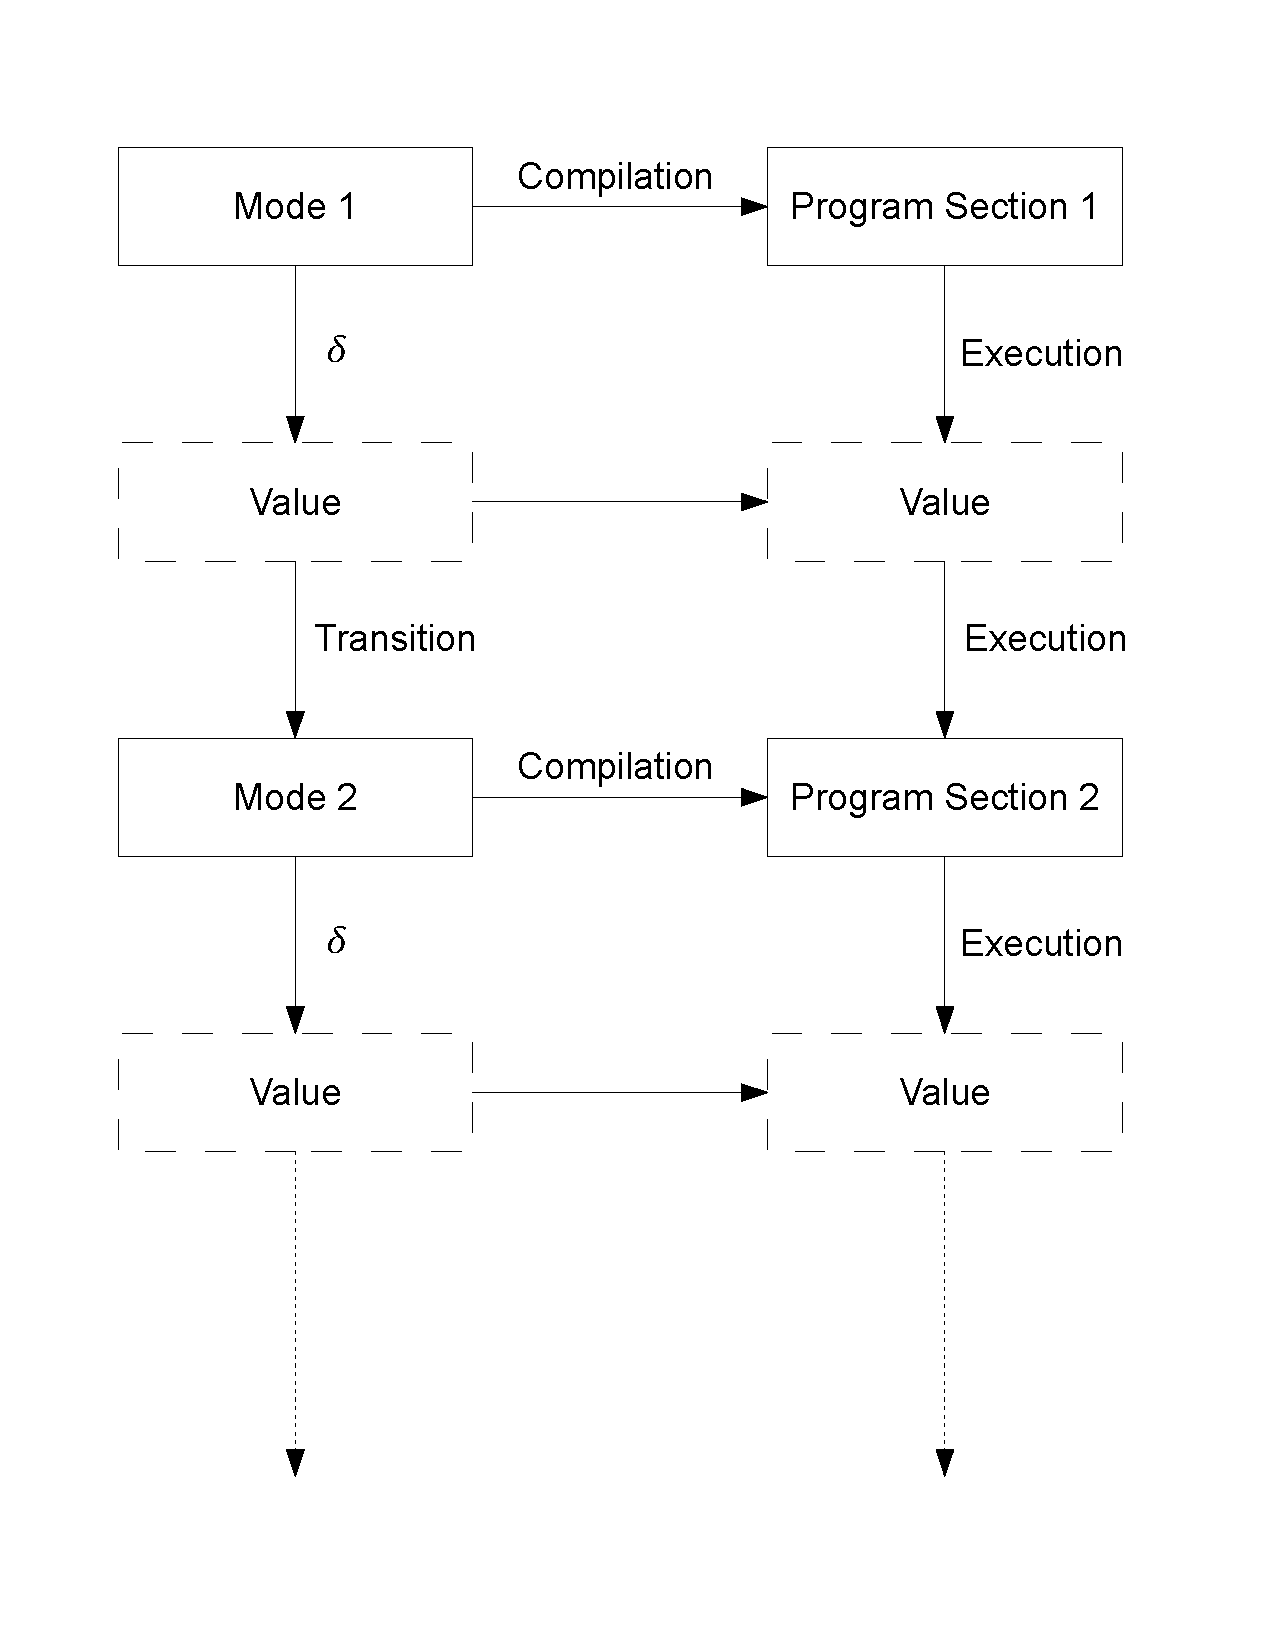
\includegraphics[trim= 10mm 30mm 10mm 10mm, clip, width=\imgmedium]{./images/correctness_graph2.pdf}
    \caption{Code Transition Structure}
    \label{fig:correctness_graph2}
\end{figure}

generated from an graph structure is correct. To do so we extend figure \ref{fig:correctness_graph1} iteratively to obtain figure \ref{fig:correctness_graph2} to evaluate the transitions.

In this section we will begin by showing that each of the transformations are correct by constructing basic atoms. We will start by looking at atoms that have the simplest expressions first. The simplest of these is a diagram in which only the start node exists as shown in \ref{fig:correctness_ex_start}.

\subsection{Correctness over Structure}
\subsubsection{Start}
\begin{figure}[htb]
	\centering
	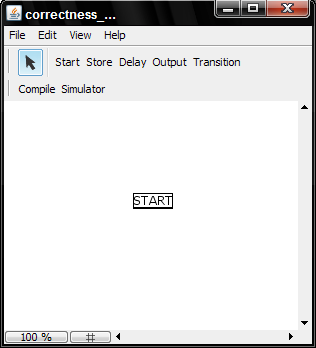
\includegraphics[width=\imgmedphoto]{./images/correctness_ex_start.png}
	\caption{Singular Start Block}
	\label{fig:correctness_ex_start}
\end{figure}
In this simple example the following generated intermediate code \emphasize{IL} is created.

\begin{minipage}{\textwidth}
\begin{lstlisting}[frame=single]
00 // BEGIN VARIABLE INITIALIZATIONS //
01 // END VARIABLE INITIALIZATIONS //
02
03 BLUID0:
04 //////////////////////////////////////
05 //        PROGRAM START             //
06 //////////////////////////////////////
07 goto EOF;
08 
09 EOF:
10 return;
\end{lstlisting}
\end{minipage}

In this simplest example we have a label inserted at the beginning of the start block so we can re-enter the start block namely BLUID0. Following the label a comment header to denote the block type, and no variables declared.  Because there is no other transition or block an automatic transition to \emphasize{EOF} is setup in order to terminate the program. In our system this is analogous to ``staying in a state indefinitely'' as the behaviour after return is executed is to just halt the chip.


\subsubsection{Delay Element}

\begin{figure}[htb]
	\centering
	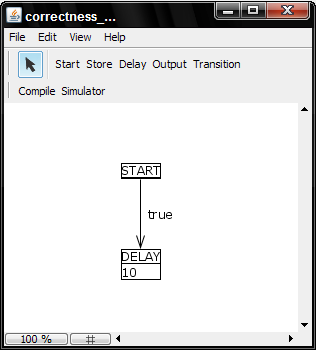
\includegraphics[width=\imgmedphoto]{./images/correctness_ex_delay.png}
	\caption{Delay Block}
	\label{fig:correctness_ex_delay}
\end{figure}

Moving up in complexity we have a start block followed by our next simplest element the delay block, joined by one transition leaving the start block. We can see from figure \ref{fig:correctness_ex_delay}
the structure of this new graph. We will use this example to examine transitions are compiled into final code, but first we shall look at the delay block itself.

\begin{minipage}{\textwidth}
\begin{lstlisting}[frame=single]
// VARIABLE INITIALIZATIONS //
...

BLUID1:
//////////////////////////////////////
//        DELAY                     //
//////////////////////////////////////
delayms(10);
goto EOF;

EOF:
return;
\end{lstlisting}
\end{minipage}

The delay block itself has a structure identical to the start block. The only difference in this case is the delay block doesn't have a null code section. The delay block generates one line of code, namely delay(integer). The actual delay routine is implemented on the driver level per device since certain devices lack internal timers. It will be up to each implementer to ensure that the delay will correctly delay each the integer specified (in milliseconds). 

\begin{minipage}{\textwidth}
\begin{lstlisting}[frame=single]
00 // BEGIN VARIABLE INITIALIZATIONS //
01 // END VARIABLE INITIALIZATIONS //
02 
03 BLUID0:
04 //////////////////////////////////////
05 //        PROGRAM START             //
06 //////////////////////////////////////
07 goto BLUID1;
08 goto EOF;
09 
10 BLUID1:
11 //////////////////////////////////////
12 //        DELAY                     //
13 //////////////////////////////////////
14 delayms(10);
15 goto EOF;
16
17 EOF:
18 return;
\end{lstlisting}
\end{minipage}

In the example shown in figure \ref{fig:correctness_ex_delay} a transition can be seen. The reader will observe that we have directly mapped each edge to a goto statement that is guarded by the guard condition on the edge itself. As defined in section \ref{sec:statechartsyn} the transitions are always mutually exclusive and to not do so would be considered a syntax error. The reason is there is no way to enforce sequence in which each edge is evaluated that would make sense to the programmer constructing the diagram in a visual way. It is up to the programmer (diagram constructor) to ensure that we never run into a condition where two edges actually have an area of overlap. This is not a problem for our simple case as shown in figure \ref{fig:correctness_ex_delay} as we only have one edge leaving the delay block.

Each block has an unique identifier associated with it, this identifier is what is used by the goto blocks in order to recreate the graph structure in the code. The unique identifier is generated at design time and is checked at compile time to ensure that it is in fact unique.

\subsubsection{Output Element}

The output block is similar to the previous delay block however the new item introduced by the output block are variables. The output block during its run will need to set a value to a variable. It does this in order to update the output on the port. 

\begin{figure}[htb]
	\centering
	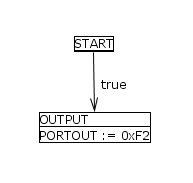
\includegraphics[width=\imgmedphoto]{./images/correctness_ex_output.png}
	\caption{Output Block}
	\label{fig:correctness_ex_output}
\end{figure}

The resulting compiled output from figure \ref{fig:correctness_ex_output} is shown below.

\begin{minipage}{\textwidth}
\begin{lstlisting}[frame=single]
00 // BEGIN VARIABLE INITIALIZATIONS //
01 // END VARIABLE INITIALIZATIONS //
02 
03 BLUID0:
04 //////////////////////////////////////
05 //        PROGRAM START             //
06 //////////////////////////////////////
07 goto BLUID1;
08 goto EOF;
09 
10 BLUID1:
11 //////////////////////////////////////
12 //        OUTPUT                    //
13 //////////////////////////////////////
14 PORTOUT = 0xF2;
15 goto EOF;
16 
17 EOF:
18 return;
\end{lstlisting}
\end{minipage}

The reader will note that we did not change any of the transitions from figure \ref{fig:correctness_ex_delay}. Despite this the BLUID's are still different. It is easy to see that the ``goto'' routing structure still behaves the same way despite having different labels. We note that the output block's ``set'' operation as shown in figure \ref{fig:correctness_ex_output} becomes translated to ``PORTOUT = 0xF2;'' in the final intermediate language code. The right hand side of the equation can be any valid expression and is not just limited to an costant as shown here. Since the right hand side is transfered verbatim into the final code what the diagram creator draws essentially becomes exactly what is written in the final code.

\subsubsection{Input Element}

Similar to the output block the input block allows you to sample the state of the input ports and store the result into a variable. The first item to the left of the diagram is the variable type. Following the variable type is the variable name. If a new variable name is specified a new entry is created in the variable initialization section. 


\begin{figure}[htb]
	\centering
	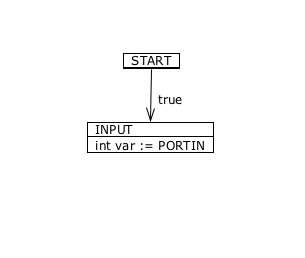
\includegraphics[width=\imgmedphoto]{./images/correctness_ex_input.png}
	\caption{Input Block}
	\label{fig:correctness_ex_input}
\end{figure}

Once again we present the compiled output for \ref{fig:correctness_ex_input} below.

\begin{minipage}{\textwidth}
\begin{lstlisting}[frame=single]
00 // BEGIN VARIABLE INITIALIZATIONS //
01 int var = 0;
02 // END VARIABLE INITIALIZATIONS //
03 
04 BLUID0:
05 //////////////////////////////////////
06 //        PROGRAM START             //
07 //////////////////////////////////////
08 goto BLUID1;
09 goto EOF;
10
11 BLUID1:
12 //////////////////////////////////////
13 //        Input                    //
14 //////////////////////////////////////
15 var = PORTIN;
16 goto EOF;
17
18 EOF:
19 return;
\end{lstlisting}
\end{minipage}

Examining the compiled code we will notice that the variable initialization section is no longer empty. Our compiler will first initialize the variable used to store the input from ``PORTIN'' to a known value. This removes any issues of unknown values from our system and as defined in section \ref{sec:statechartsem} variables all have by definition an initial set of values they take on. In the code section of our ``Input'' block we can see that our ``var := PORTIN'' becomes ``var = PORTIN;'' in the final compiled code. The left hand side var is limited to simple variables and expressions are not allowed. Once again like the previous example the data from the input diagram is transfered verbatim into the final code there by ensuring correctness.

\subsubsection{Store Element}

In order to examine transitions in more detail we need to look at logic on transitions. So far because all transitions have been guarded with he condition ``true'' or always taken we have not had the opportunity to see any guard conditions in the code. Instead in the our current code we only observe a always taken goto statement at the end. We will construct a basic diagram with our next component the ``Store Block'' to demonstrate how guard conditions are enumerated as well as demonstrate another basic primitive block that allows the diagram creator to set internal variables and perform calculations.

\begin{figure}[htb]
	\centering
	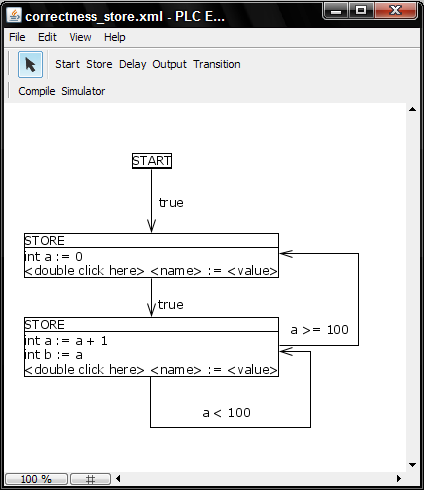
\includegraphics[width=\imgmedphoto]{./images/correctness_ex_store.png}
	\caption{Store Block Example}
	\label{fig:correctness_ex_store}
\end{figure}

The resulting code from figure \ref{fig:correctness_ex_store} is shown below:

\begin{minipage}{\textwidth}
\begin{lstlisting}[frame=single]
00 // BEGIN VARIABLE INITIALIZATIONS //
01 int a = 0;
02 int b = 0;
03 // END VARIABLE INITIALIZATIONS //
04
05 BLUID0:
06 //////////////////////////////////////
07 //        PROGRAM START             //
08 //////////////////////////////////////
09 goto BLUID1;
10 goto EOF;
11
12 BLUID1:
13 //////////////////////////////////////
14 //        STORE                     //
15 //////////////////////////////////////
16 a = 0;
17 
18 goto BLUID2;
19 goto EOF;
20
21 BLUID2:
22 //////////////////////////////////////
23 //        STORE                     //
24 //////////////////////////////////////
25 a = a + 1;
26 b = a;
27
28 if (a >= 100) goto BLUID1;
29 if (a < 100) goto BLUID2;
30 goto EOF;
31
32 EOF:
33 return;
\end{lstlisting}
\end{minipage}

First we look at the first store block with ``BLUID1'' as its label. We can easily see that from our diagram
of transformations in figure \ref{fig:correctness_graph1} that our expression ``$a := 0$'' through the compile
transformation was converted to ``$a = 0$''. Taking the transformation in figure \ref{fig:correctness_graph1}
of ``$\delta$'' we note that the meaning of ``$a := 0$'' is that the value of $\delta(a) = 0$. Similarily
executing ``$a = 0$'' in C we find that after execution the value of $exec(a) = 0$. Since the mapping from
our semantic ``value'' to our executed ``value'' is the same we can conclude that the mapping is correct as
by our definition. Next we the second store block with ``BLUID2'' as its label. From the diagram in figure
\ref{fig:correctness_ex_store} the second store block has two notable differences. The first is that it has
more than one set operation, and the second is that it uses variables in its expression and not just constants.
As stated before the right hand side allows for any expression to be placed. From our definitions in
section \ref{sec:statechartsem} of \plcchart it is understood that each expression forumlae is understood
to occur in sequence. In this example ``$a := a + 1$'' will occur before ``$b := a$''. To demonstrate
correctness we once again refer to figure \ref{fig:correctness_graph1} and start with our first expression.
We note that after compilation $a := a + 1$ is compiled to $a = a + 1$, and $b := a$ becomes $b = a$. We
can see that $\delta(a) = a + 1, \delta(b) = a + 1$, similarly $exec(a) = a + 1, exec(b) = a + 1$. Since
mapping from $\delta(a) \rightarrow exec(a)$ and $\delta(b) \rightarrow exec(b)$ we can conclude that the
transformation preserves the meaning of the values and thus is correct to the semantics outlined in
section \ref{sec:statechartsem}.

To show the correctness of guarded transitions we now look at figure \ref{fig:correctness_graph2}.
Note that figure \ref{fig:correctness_graph2} shares most of it's structure with
figure \ref{fig:correctness_graph1} but is annotated to include transitions and modes.
A mode as established in section \ref{sec:statechartsem} is similar to a state or a block in our diagram.
Our diagrams always begin from the ``start'' node, similarily our begins its execution from ``BLUID0'' in
the above code which is the compiled code. No values are updated in our start block so we can take the
transition leaving the start node this puts us into the first store block (which we will refer
to as $Store_1$ for disambiguity). On the execution side we see that at the end of the start code
block we have the line \texttt{goto BLUID1;} we can note that BLUID1 points to the code block for
our store in the diagram. We can conclude that $Transition(Start, true) \rightarrow Store_1$ similarily
$Execution(Start, true) \rightarrow Store_1$. Thus we can conclude that transitions leaving ``start'' are
correct. A similar argument can be made for $Store_1$ since no transitions are guarded.

For the guarded transitions in our second store block which we will refer to as $Store_2$ with
``BLUID2'' we must look at each guarded condition. We have previously shown for
figure \ref{fig:correctness_ex_store} that figure \ref{fig:correctness_graph1} holds
so we will skip showing it again here. Extracting all edges leaving $Store_2$ we
obtain $Transition(Store_2, a >= 100) \rightarrow Store_1$ and $Transition(Store_2, a < 100) \rightarrow Store_2$.
Now all that remains is to show that the execution code has the same transitions.
We can see from the compiled code that at the end of our $Store_2$ code block we have
a series of ``if'' statements. We can see that \texttt{if (a >= 100) goto BLUID1;} is
equivalent to $Transition(Store_2, a >= 100) \rightarrow Store_1$ and \texttt{if (a < 100) goto BLUID2;} is
equivalent to $Transition(Store_2, a < 100) \rightarrow Store_2$. In this way we
have demonstrated that guarded conditions are correct as well.

By demonstrating that our system is correct both in compilation and the structure execution
with respect to figures \ref{fig:correctness_graph1} and \ref{fig:correctness_graph2}. We can
conclude that our system is functionally correct by its construction and structure. To fully
justify the correctness of the system we still need to show execution traces of each of the
examples shown in this section. In the next section we will demonstrate execution traces
of each diagram.


\subsection{Correctness over Execution}
\subsubsection{Table Representation}

In order to show the correctness of the execution it is necessary to identify the differences between graphical traces and execution. Both contain a ``mode'' however in execution the mode can be directly accociated to a set of line numbers. Line numbers don't exist in the diagram view. Both however do have variables and modes, and correct execution is a trace where all modes and variables are identical.

\begin{table}[htcb]
	\caption{Start Diagram shown in figure \ref{fig:correctness_ex_start}}
	\centering
		\begin{tabular}{| l | l | l | l |}
			\hline
			\textbf{Mode} & \textbf{Variables} & \textbf{Transitions} & \textbf{Next Mode} \\
			\hline
			start & (none) & (none) & (none meaning stop) \\
			\hline
			(none) & (none) & (none) & (none) \\
			\hline
		\end{tabular}
	\label{table:BasicDiagOnly}
\end{table}

To show an execution trace we replace mode with line number and we get the following table.

\begin{table}[htcb]
	\caption{Start code execution for compiled code from diagram \ref{fig:correctness_ex_start}}
	\centering
		\begin{tabular}{| l | l | l | l |}
			\hline
			\textbf{Line} & \textbf{Variables} & \text{Code} & \textbf{Next Executed Line} \\
			\hline
			00 & (none) & (comment) & 07 \\
			\hline
			07 & (none) & \texttt{goto EOF} & 09 \\
			\hline
			09 & (none) & (line label) & 10 \\
			\hline
			10 & (none) & return & (stop) \\
			\hline
		\end{tabular}
	\label{table:BasicExecOnly}
\end{table}

It is not to difficult to see that from lines 00 to 07 we are in the ``start'' mode so we can append a
mode marker to the end of the table. We can also identify that line 09 ``EOF'' represents the end of the
file and thus has no mode accociated with it or goes to a null mode.

\begin{table}[htcb]
	\caption{Start code execution for compiled code from diagram extended\ref{fig:correctness_ex_start}}
	\centering
		\begin{tabular}{| l | l | l | l | l |}
			\hline
			\textbf{Line} & \textbf{Variables} & \textbf{Code} & \textbf{Next Executed Line} & \textbf{Mode}\\
			\hline
			00 & (none) & (comment) & 07 & \textbf{start} \\
			\hline
			07 & (none) & \texttt{goto EOF} & 09 &  \textbf{start}\\
			\hline
			09 & (none) & (line label) & 10 & \textbf{none} \\
			\hline
			10 & (none) & return & (stop) & \textbf{none} \\
			\hline
		\end{tabular}
	\label{table:BasicExecMode}
\end{table}

We can already see that the two traces produce the same outcome however for ease of comparison we can
merge the two tables side by side so we can directly compare each executed line to it's accocated graph.

\begin{table}[htcb]
	\caption{Start code execution combined table. For figure \ref{fig:correctness_ex_start}}
	\centering
	\tablefontsize
		\begin{tabular}{| p{0.06\textwidth} | p{0.1\textwidth} | p{0.15\textwidth} | p{0.06\textwidth} | p{0.05\textwidth} | p{0.1\textwidth} | p{0.2\textwidth} | p{0.07\textwidth} |}
			\hline
			\textbf{Mode} 		&	\textbf{Var (Diag)} 		& 	\textbf{Transitions} 		& 	\textbf{Next}		&	\textbf{Line}		&	\textbf{Var (Exec)	}	&	\textbf{Code}	&	\textbf{Next LN} \\
			\hline
			start 				&	(none)						&	(none)						&	(none meaning stop)	&	00					&	(none)					& 	(comment)		&	07 \\
			\hline
								&								&								&						&	07					& 	(none)					& 	goto EOF		& 	10 \\
			\hline
								&								&								&						&	10					&	(none)					&	return			&	(stop) \\
			\hline
		\end{tabular}
	\label{table:BasicExecCombined}
\end{table}

In table \ref{table:BasicExecCombined} we can easily compare the combined execution vs the diagram code trace. 
We can see that line numbers can be accociated with a mode dispite not having one themselves. In order to verify 
correct execution it is necessary to show that the sequence of modes and values are the same. In the above example
 in which we run our first trivially simple start code snippet it is easy to see that this holds. Therefore we can
  conclude that the execution is correct for the start diagram shown in figure \ref{fig:correctness_ex_start}.

\subsubsection{Start Diagram Execution}

Please see table \ref{table:BasicExecCombined}. We may note that the only mode is ``start'' and that the mode
is followed through the executed line by line trace. We can also note that the code stops after ``start'' 
mode is finished which also is correct behavior. Finally we can note that there are no varibles listed in
our system so both sets of variables are trivially correct.

\subsubsection{Delay Diagram Execution}

\begin{table}[htcb]
	\caption{Delay code execution combined table. For figure \ref{fig:correctness_ex_delay}}
	\centering
	\tablefontsize
		\begin{tabular}{| p{0.06\textwidth} | p{0.1\textwidth} | p{0.15\textwidth} | p{0.06\textwidth} | p{0.05\textwidth} | p{0.1\textwidth} | p{0.2\textwidth} | p{0.07\textwidth} |}
			\hline
			\textbf{Mode} 		&	\textbf{Var (Diag)} 		& 	\textbf{Transitions} 		& 	\textbf{Next}		&	\textbf{Line}		&	\textbf{Var (Exec)	}	&	\textbf{Code}	&	\textbf{Next LN} \\
			\hline
			start 				&	(none)						&	if (true) delay				&	delay				&	00					&	(none)					& 	(comment)		&	07 \\
			\hline
								&								&								&						&	07					& 	(none)					& 	goto BLUID1		& 	10 \\
			\hline
			delay				&	(none)						&	(none)						&	(stop)				&	10					&	(none)					&	(line label)	&	14 \\
			\hline
								&								&								&						&	14					&	(none)					&	delayms(10)		&	15 \\
			\hline
								&								&								&						&	15					&	(none)					&	goto EOF		&	17 \\
			\hline
								&								&								&						&	17					&	(none)					&	(line label)	&	18 \\
			\hline
								&								&								&						&	17					&	(none)					&	return			&	(stop) \\
			\hline
		\end{tabular}
	\label{table:DelayExecCombined}
\end{table}

Once again in this example we don't have any variable so they are easily verified by checking that in both cases
there are no variables. All that's left to justify correctness is ensuring the sequence of modes is executed correctly.
It should be easy to see that the sequence: start, delay, stop. Is clearly implimented by the executed code from the table
\ref{table:DelayExecCombined}. We can therefor conclude that the excuted code trace is correct with respect to the original
diagram.

\subsubsection{Output Diagram Execution}

\begin{table}[htcb]
	\caption{Output code execution combined table. For figure \ref{fig:correctness_ex_output}}
	\centering
	\tablefontsize
		\begin{tabular}{| p{0.05\textwidth} | p{0.1\textwidth} | p{0.14\textwidth} | p{0.05\textwidth} | p{0.05\textwidth} | p{0.12\textwidth} | p{0.2\textwidth} | p{0.07\textwidth} |}
			\hline
			\textbf{Mode} 		&	\textbf{Var (Diag)} 		& 	\textbf{Transitions} 		& 	\textbf{Next}		&	\textbf{Line}		&	\textbf{Var (Exec)	}	&	\textbf{Code}	&	\textbf{Next LN} \\
			\hline
			start 				&	PORTOUT = 0					&	if (true) output			&	output				&	00					&	PORTOUT = 0				& 	(comment)		&	07 \\
			\hline
								&								&								&						&	07					&   PORTOUT = (no change)	&	goto BLUID		&	10 \\
			\hline
			output				&	PORTOUT = 0xF2				&	(none)						&	(stop)				&	10					&	PORTOUT = (no change)	&	(line label)	&	14 \\
			\hline
								&								&								&						&	14					&	PORTOUT = 0xF2			&	PORTOUT = 0xF2	&	15 \\
			\hline
								&								&								&						&	15					&	PORTOUT = (no change)	&	goto EOF		&	17 \\
			\hline
								&								&								&						&	17					&	PORTOUT = (no change)	&	(line label)	&	18 \\
			\hline
								&								&								&						&	18					&	PORTOUT = (no change)	&	return			&	(stop) \\
			\hline
		\end{tabular}
	\label{table:DelayExecCombined}
\end{table}

First we make a note that PORTOUT is an special variable that is used to send an output to the ports on the device.
According to the hardware specification section PORTOUT is initialized to 0 when the device first starts up.
Likewise PORTOUT is zero until changed in our diagram. In understanding this the rest of the code trace is as follows:
\{(start, PORTOUT = 0), (output, PORTOUT = 0xF2)\} where we observe that our tuple comprises of (mode, variables). 
It is not difficult to see that our two code traces produce this sequence and by our definition we can conclude that our
output execution is correct with respect to the diagram.


\subsubsection{Input Diagram Execution}

\begin{table}[htcb]
	\caption{Input code execution combined table. For figure \ref{fig:input_ex_output}}
	\centering
	\tablefontsize
		\begin{tabular}{| p{0.05\textwidth} | p{0.1\textwidth} | p{0.14\textwidth} | p{0.05\textwidth} | p{0.05\textwidth} | p{0.12\textwidth} | p{0.2\textwidth} | p{0.07\textwidth} |}
			\hline
			\textbf{Mode} 		&	\textbf{Var (Diag)} 		& 	\textbf{Transitions} 		& 	\textbf{Next}		&	\textbf{Line}		&	\textbf{Var (Exec)	}	&	\textbf{Code}	&	\textbf{Next LN} \\
			\hline			
								&								&								&						&	00					& 	var = UNDEFINED			&	(comment)		&	01	\\
			\hline
								&								&								&						&	01					&	var = 0					&	int var = 0		&	04	\\
			\hline
			start 				&	var = 0						&if (true) $\rightarrow$ input	&	input				&	04					&	var = (no change)		& 	(comment)		&	08	\\
			\hline
								&								&								&						&	08					&	var = (no change)		&	goto BLUID1		&	11	\\
			\hline
			input				&	var = PORTIN				&	(none)						&	(stop)				&	11					&	var = (no change)		&	(line label)	&	15	\\
			\hline
								&								&								&						&	15					&	var = PORTIN			&	var = PORTIN	&	16	\\
			\hline
								&								&								&						&	16					&	var = (no change)		&	goto EOF		&	18	\\
			\hline
								&								&								&						&	18					&	var = (no change)		&	(line label)	&	19	\\
			\hline
								&								&								&						&	19					&	var = (no change)		&	return			&	(stop)	\\
			\hline
		\end{tabular}
	\label{table:InputExecCombined}
\end{table}

